\documentclass[runningheads]{llncs}
\usepackage{graphicx}
\usepackage{url}
% Used for displaying a sample figure. If possible, figure files should
% be included in EPS format.
%
% If you use the hyperref package, please uncomment the following line
% to display URLs in blue roman font according to Springer's eBook style:
% \renewcommand\UrlFont{\color{blue}\rmfamily}

\begin{document}
\title{MongoDB for Credit Card Fraud Detection}

\author{Davide Cazzetta\orcidID{976585} \and Riccardo Giussani\orcidID{000000}}

\authorrunning{Davide \& Riccardo}
% First names are abbreviated in the running head.
% If there are more than two authors, 'et al.' is used.
%
\institute{Università degli Studi di Milano Statale, Milan MI 20133, Italy \\
\url{https://www.unimi.it/it/corsi/corsi-di-laurea/informatica-magistrale}}
%
\maketitle              % typeset the header of the contribution
%
\begin{abstract}
The abstract should briefly summarize the contents of the paper in
150--250 words.

\keywords{First keyword  \and Second keyword \and Another keyword.}
\end{abstract}

\section{Introduction}

\subsection{Motivation}

Payment card fraud is a major challenge for business owners, payment card issuers, and transactional services companies, causing every year substantial and growing financial losses. Many Machine Learning approaches have been proposed in the literature that tries to automate the process of identifying fraudulent patterns from large volumes of data. The focus of this project aims at this last part: we exploit some algorithms that generate data about transactions to store these data into a NoSQL Database, specifically MongoDB\footnote{https://www.mongodb.com/}. In detail we want to see how does this system behave in the presence of large amount of data, evaluating the execution times for some operations.

\subsection{Conceptual Model}

\begin{enumerate}
    \item ref allo script e due parole sul problema
    \item UML, constraints e supposizioni
\end{enumerate}
explanations, motivations, constraints, and any other information that allows understanding the design carried out.
\\
\begin{figure}[!htb] 
        \centering 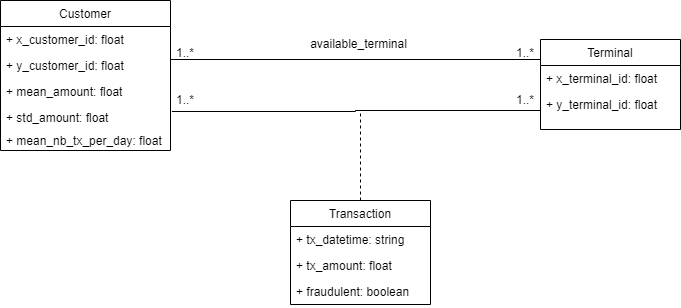
\includegraphics[width=0.9\columnwidth]{images/FraudDetectionUML.png}
        \caption{\label{fig1}Questo è UML dei dati come vengono generati dallo script}
\end{figure}
Come detto ci sono due entità, \textbf{Customer} e \textbf{Terminal}, con la relazione \textbf{Transaction}.
\\
CERCA QUESTIONE ID
\\
Teniamo fissi Customer e Terminal (?)
\\
Tra Customer e Terminal esiste anche la relazione \textbf{available terminal}
\\
In un ipotetico DB relazionale, avrei la tabella \textbf{Transaction} che funge da join table tra Customer e Terminal.
\\
Constraints e supposizioni:
\begin{enumerate}
    \item può sussistere una transaction tra un customer e un terminal se e solo se sussiste tra quei due anche la relazione \textbf{available terminal}
    \item può sussistere la relazione \textbf{available terminal} tra customer e terminal se e solo se il punto in cui si trova terminal è entro un certo raggio dalle coordinate di customer
    \item le coordinate geografiche sono tra 0 e 100
    \item datetime è una stringa conforme
    \item fraudulent è un boolean che dobbiamo calcolare noi
\end{enumerate}

\section{Logical Model}
\subsection{Baseline Model}
Essendo Transactions un'entità centrale, scegliamo di trattarla come entità (nel senso, è una relazione ma è molto importante)\\
\begin{figure}[!htb] 
        \centering 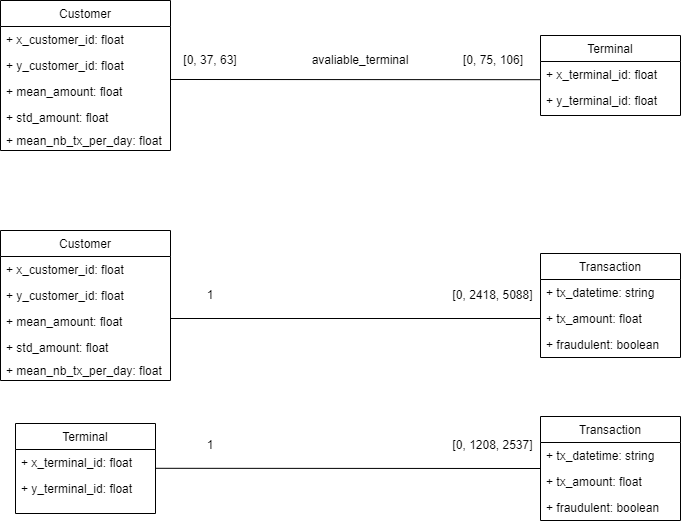
\includegraphics[width=0.9\columnwidth]{images/MongoCardinality.png}
        \caption{\label{fig2}Cardinalità delle relazioni; va bene così perchè card C-T è diversa da quella T-T}
\end{figure}
Queries tell us how we should navigate relationships:
\begin{enumerate}
    \item[a)] requires navigability from Customer to Transaction, to compute the sum
    \item[b)] requires to navigate from terminal to transaction, in order to compute the average, then from transaction to terminal in order to mark fraudulent transactions
    \item[c)] requires to navigate from customer to terminal: we check for customers all terminals used in at least a transaction and then lookup for other customers that allow us to do the chain
    \item[d)] only requires transactions data, and also to generate a new collection, which will navigate from buyingFriends to Customer (we'll see the cardinality). buyingFriends is transitive !
    \item[e)] only requires transactions data
\end{enumerate}
NOTA: i dati di terminal non sono mai acceduti, quindi se ne stanno in una collezione loro e uso solo ref.
\\
The logical data model that has been realized for addressing the requirements imposed by the proposed operations. It is mandatory the presence of the motivations that led to the generation of the data model.
provide a data modeling to optimize the execution of the following operations
\begin{figure}[!htb] 
        \centering 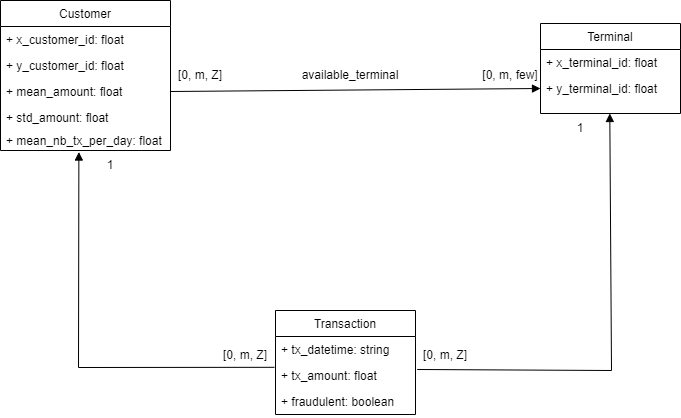
\includegraphics[width=0.9\columnwidth]{images/MongoBaselineNavigability.png}
        \caption{\label{fig3}Questa è la navigabilità baseline, solo guardando le query. Poi bisogna vedere le cardinalità}
\end{figure}
Considerazioni:
\begin{enumerate}
    \item navigation from customer to transaction is impractical: ZILLIONS!
    \item navigation from terminal to transaction is impractical: ZILLIONS!
\end{enumerate}
So we ignore these and just keep navigability from transaction to customer and from transaction to terminal\\
We just navigate from transactions to the other two, do things through a lookup (\textbf{in the baseline case!})
\subsection{Design Patterns}
\textbf{Prima eseguiremo le query sulle collezioni base, poi su quelle ottimizzate coi design pattern per far vedere che si va a migliorare}

\section{Ingestion Layer}

The ingestion layer is responsable for generating the datasets which will then be stored in MongoDB.

\subsection{Generate datasets}

The system can generate three datasets, one about customers, one related to terminals and the third regarding transactions. To generate these datasets we have exploited the scripts presented in this article: \url{fraud-detection-handbook.github.io/fraud-detection-handbook/Chapter_3_GettingStarted/SimulatedDataset.html}. In particular we have created a class \emph{DatasetsGenerator} where the user can pass the parameters \emph{start\_date} which represents the day on which transactions begin and \emph{nb\_days}, that is days of transactions. The decision to make only these two parameters arbitrary is due to the fact that the biggest dataset is about transactions, on the other hand the customers and terminals dataset are are much smaller in comparison, as a result, the customer and terminal parameters are constant at 5000 and 10000 respectively.
\\
The objective of the work is to generate three datasets each composed of the three datasets described above, to do this we started with a base of 5000 customers, 10000 terminals and 180 days of transactions (starting from the date 2018-04-01) and then, at each iteration, the start date is increased by one year and the days of transactions are doubled. The following datasets were generated in this way:

\begin{enumerate}
    \item \begin{itemize}
        \item customers: 3 MB
        \item terminals: 1 MB
        \item transactions (2018): 330 MB
    \end{itemize}
    \item \begin{itemize}
        \item customers: 3 MB
        \item terminals: 1 MB
        \item transactions (2019): 670 MB
    \end{itemize}
    \item \begin{itemize}
        \item customers: 3 MB
        \item terminals: 1 MB
        \item transactions (2020): 1.3 GB
    \end{itemize}
\end{enumerate}

\subsection{Store data in MongoDB}

The second part of the ingestion layer consists of saving the data in MongoDB. The datasets are generated in json format to facilitate saving in the database; in fact the data are stored with the \emph{updateMany\footnote{https://docs.mongodb.com/manual/reference/method/db.collection.updateMany/}} method. In particular, transaction data are saved at each iteration, whereas customer and terminal datasets are only saved at the first iteration as they are the same for all three generated datasets.

\subsubsection{Design Patterns}

\section{Queries}

This section explains in detail how the queries were implemented to obtain the required results.

\subsection{Query A}

For each customer identifies the amount that he/she has spent for every day of the current month.

\subsection{Query B}
\subsection{Query C}
\subsection{Query D}
Ci viene richiesta una nuova relazione
\begin{figure}[!htb] 
        \centering 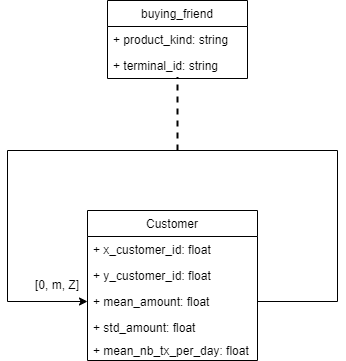
\includegraphics[width=0.5\columnwidth]{images/buyingFriends.png}
        \caption{\label{fig4}Relationship}
\end{figure}
Notare che è \textbf{transitiva} dunque basta capire per ogni customer su quali terminal ha effettuato più di 3 transazioni dello stesso tipo, poi segnalarlo
\subsection{Query E}

\section{Performance}
Valutazione performance, sia nel caso naive che nel caso ottimizzato coi pattern

\section{Conclusion}
This section should be brief, concise, but complete. Directly answer your objectives, state your findings with errors, and conclude whether or not you were successful. Briefly explain if not successful.

\end{document}
